The tool is build using rascal. The tool is build under the assumption that the library are functionally correctly under normal usage.

\section*{Abstract syntax tree}
The abstract syntax tree contains information about all types contained in the project. The information is presented as a tree with nodes and children. Using this abstract syntax tree all variable and return types can be extracted. These are then displayed in the class diagram.

\section*{M3 Model}
The M3 model is a wrapper around the abstract syntax tree. Using the m3 all information about classes like class names, methods, etc can be acquired. This information is presented as a set of functions with annotations. The M3 contains the same information as the abstract syntax tree however class information can easier be deduced from the M3.

\section*{Object Flow Diagram}
An object flow is a path along objects of data that gets passed. The object flow is represented as a relation between object calls, assigns and data. The dependencies between object are deduced from the object flow graph.

\begin{figure}[h!]
  \begin{center}
    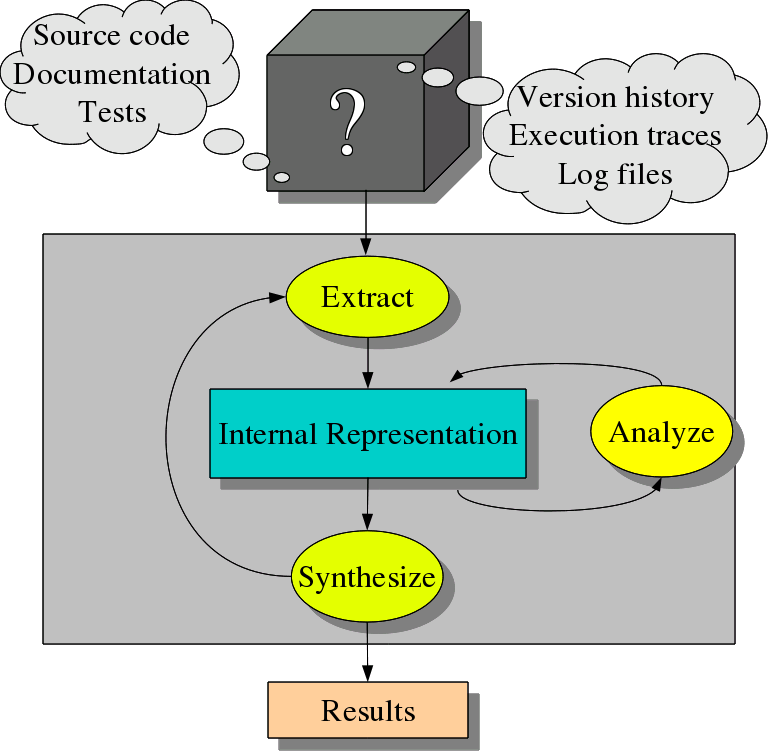
\includegraphics[width=0.48\textwidth]{figures/easy-workflow.png}
  \end{center}
  \caption{Extract-Analyze-Synthesize (EASY) paradigm}
\end{figure}

\section*{Visualization}
All the acquired information is used to generate a dot file. The dot file contains the class information added with graphical styles. Using graphviz the class diagram can be generated from the dot file.

\section*{Usage}
The tool chain can be used to reverse engineer and generate the documentation like class and flow diagrams directly from java programs. The tool works best on small to medium size projects, since the visualization of class diagram in larger projects should be partitioned in smaller sub diagrams. This functionality is not supported in the current version of the tool. 